% !TEX program = xelatex
\documentclass[UTF8,a4paper,12pt,fontset=windows]{ctexart}

\usepackage[a4paper,top=2.35cm,bottom=2.25cm,left=2.55cm,right=2.55cm]{geometry}
\usepackage{fontspec}
\setmainfont{Times New Roman}
\setCJKmainfont{SimSun}
\setCJKsansfont{Microsoft YaHei}
\usepackage{amsmath,amssymb,bm}
\usepackage{booktabs,tabularx,array,longtable,threeparttable}
\usepackage{graphicx,float,caption,subcaption}
\usepackage{siunitx}
\usepackage{enumitem}
\usepackage{setspace}
\usepackage{fancyhdr}
\usepackage[hidelinks]{hyperref}
\usepackage{bookmark}
\usepackage{url}

\graphicspath{{assets/}}
\sisetup{detect-all,per-mode=symbol}
\setstretch{1.32}
\setlength{\parindent}{2em}
\setlength{\parskip}{0.22em}
\setlength{\tabcolsep}{5pt}
\renewcommand{\arraystretch}{1.22}
\captionsetup{font=small,labelsep=quad,justification=centering}
\setlist[itemize]{leftmargin=2em,itemsep=0.25em,topsep=0.4em}
\setlist[enumerate]{leftmargin=2.3em,itemsep=0.35em,topsep=0.4em}

\ctexset{
  section={format=\heiti\zihao{3},beforeskip=1.7ex,afterskip=1.0ex},
  subsection={format=\heiti\zihao{4},beforeskip=1.25ex,afterskip=0.65ex},
  subsubsection={format=\heiti\zihao{-4},beforeskip=1.0ex,afterskip=0.5ex}
}

\pagestyle{fancy}
\fancyhf{}
\fancyhead[L]{\small 无人机编队智能避障项目技术报告}
\fancyhead[R]{\small V1.1.1}
\fancyfoot[C]{\thepage}
\renewcommand{\headrulewidth}{0.35pt}
\renewcommand{\footrulewidth}{0pt}
\setlength{\headheight}{15pt}

\newcolumntype{Y}{>{\raggedright\arraybackslash}X}
\newcolumntype{C}[1]{>{\centering\arraybackslash}p{#1}}
\newcommand{\code}[1]{\texttt{#1}}

\begin{document}

\begin{titlepage}
  \thispagestyle{empty}
  \centering
  \vspace*{3.1cm}
  {\heiti\zihao{0} 无人机编队智能避障项目技术报告\par}
  \vspace{1.1cm}
  {\songti\zihao{2} 项目原理、实现方法与性能评估\par}
  \vspace{2.3cm}
  \rule{0.72\textwidth}{0.5pt}\par
  \vspace{1.2cm}
  \begin{tabular}{@{}rl@{}}
    软件版本： & V1.1.1 \\
    源码提交： & \code{5f5b69c} \\
    评估样本： & 固定 seed 1--200 \\
    仿真平台： & MATLAB R2024a \\
    建模范围： & 二维质点编队与静态圆形障碍 \\
  \end{tabular}
  \vfill
  {\zihao{4} 2026 年 9 月 22 日\par}
\end{titlepage}

\pagenumbering{Roman}

\begin{abstract}
本项目研究五架无人机在二维随机静态障碍环境中的编队避障问题。系统采用领航--跟随结构：长机利用膨胀栅格路径规划与改进人工势场完成导航，僚机沿长机历史轨迹跟随，并在终端恢复固定 V 形；Actor--Critic 自适应动态规划提供在线加速度修正，预测式安全层负责连续扫掠避碰。当前版本最大速度为 \SI{4.5}{m/s}，长机规划净空为 \SI{4.2}{m}。

本报告直接基于 F 盘 V1.1.1 源码重新运行 seed 1--200。共 197 个 seed 成功、2 个碰撞、1 个超时，样本成功率为 98.5\%，Wilson 95\% 区间为 95.68\%--99.49\%。成功样本平均完成时间为 \SI{28.74}{s}，长机平均路径为 \SI{87.72}{m}，相对 \SI{79.40}{m} 直线距离增加 10.5\%。成功 seed 的最后 \SI{1}{s} 队形误差 RMS 均值为 \SI{0.062}{m}，但巡航阶段达到 \SI{8.59}{m}，说明当前系统能在终点准确归队，却没有在全航程严格保持几何 V 形。

局部线性分析表明，在无障碍、未饱和、参考固定且 ADP 修正冻结的条件下，僚机编队 PD 子系统与长机保持子系统均为 Hurwitz 稳定。完整系统包含势场、输入限幅、航点与模式切换、非光滑安全修正和在线学习，因此现阶段只能报告局部稳定性与样本收敛证据，不能宣称全局渐近稳定。

\noindent\textbf{关键词：}无人机编队；人工势场；自适应动态规划；路径规划；避碰；闭环稳定性
\end{abstract}

\clearpage
\begingroup
\small
\setstretch{1.0}
\tableofcontents
\endgroup
\clearpage
\pagenumbering{arabic}

\section{项目概况}

\subsection{研究目标}

项目目标是在随机静态障碍物环境中，让 1 架长机和 4 架僚机从起点区域飞到目标区域，避免无人机与障碍物碰撞以及机间碰撞，并在任务末端恢复 V 形队列。系统同时考察到达效率、避障路径代价、队形保持误差、闭环收敛、速度与加速度约束，以及不同随机场景下的成功率。

当前版本恢复了 V1.1.0 的领航--跟随编队控制，把最大速度调整为 \SI{4.5}{m/s}，长机规划的障碍膨胀净空保持为 \SI{4.2}{m}。报告对应 Git 提交 \code{5f5b69c}。

\subsection{系统边界与默认参数}

\begin{table}[H]
\centering
\caption{项目默认运行条件}
\label{tab:scope}
\begin{tabularx}{0.93\textwidth}{@{}lY@{}}
\toprule
项目 & 当前设置 \\
\midrule
无人机模型 & 二维单位质量质点，状态为位置与速度 \\
编队规模 & 5 架无人机，1 号机为长机 \\
起点与目标 & 长机从 $(10,10)\,\mathrm{m}$ 飞向 $(70,62)\,\mathrm{m}$ \\
工作空间 & \SI{80}{m}$\times$\SI{80}{m} \\
障碍物 & 8 个静态圆，半径 \SIrange{1.2}{2.6}{m} \\
时间离散 & $\Delta t=\SI{0.05}{s}$，最大仿真时间 \SI{500}{s} \\
运动限制 & 最大速度 \SI{4.5}{m/s}，最大加速度 \SI{3.0}{m/s^2} \\
编队几何 & 排间纵向距离 \SI{3.0}{m}，每排横向偏移 \SI{2.5}{m} \\
\bottomrule
\end{tabularx}
\end{table}

\section{系统模型与基本原理}

\subsection{运动模型与任务状态}

第 $i$ 架无人机采用二阶质点模型。控制器输出二维加速度，随后经限幅并用显式欧拉法推进状态：
\begin{equation}
\dot{\bm p}_i=\bm v_i,\qquad
\dot{\bm v}_i=\bm u_i,\qquad
\lVert\bm v_i\rVert\leq \SI{4.5}{m/s},\qquad
\lVert\bm u_i\rVert\leq \SI{3.0}{m/s^2}.
\end{equation}

任务成功要求同时满足：长机到目标距离不大于 \SI{1}{m}；四架僚机的最大队形误差不大于 \SI{1}{m}；全机最大速度不大于 \SI{0.25}{m/s}；上述条件连续保持 \SI{1}{s}；此前未发生碰撞且总时间未超过 \SI{500}{s}。

\subsection{控制与规划链路}

\begin{table}[H]
\centering
\caption{控制与规划链路}
\label{tab:pipeline}
\small
\begin{tabularx}{\textwidth}{@{}C{2.0cm}C{3.0cm}YC{2.7cm}@{}}
\toprule
阶段 & 输入 & 主要处理 & 输出 \\
\midrule
场景生成 & seed 与障碍参数 & 圆障碍采样、整队净空可行性过滤 & 可复现障碍集合 \\
长机规划 & 起点、目标、障碍 & 膨胀栅格建图、最短路与视线简化 & 长机航点序列 \\
编队参考 & 长机历史轨迹 & 按弧长滞后并叠加横向偏移 & 僚机期望状态 \\
基础控制 & 位置速度误差 & 目标制导、APF、编队 PD 与机间斥力 & 基础加速度 \\
ADP 修正 & 风险与状态特征 & Actor 输出，Critic 与 Actor 在线更新 & 自适应加速度 \\
安全层 & 当前状态与候选控制 & 制动约束与最多 5 次扫掠预测修正 & 最终受限控制 \\
终止判定 & 目标、队形、速度、碰撞 & 连续保持或碰撞、超时判定 & 成功或失败原因 \\
\bottomrule
\end{tabularx}
\end{table}

\subsection{人工势场与路径规划}

长机先在 \SI{1}{m} 分辨率的 $81\times81$ 栅格中规划路径。障碍物半径在长机建图时增加 \SI{4.2}{m}；若起点到目标的线段已经满足净空，则直接采用目标点，否则构造八邻接可行图，求最短路径并用可见性检查简化航点。在线阶段，目标引力按剩余距离生成期望速度，障碍斥力在距表面 \SI{6}{m} 内起作用，并加入切向分量以降低局部极小问题。障碍风险越高，控制器越多地把权重交给斥力。

需要区分两个净空口径。长机路径规划函数直接使用 \SI{4.2}{m}；随机场景生成器为了保证整队可通行，会取 \SI{4.2}{m} 与“最大横向偏移 \SI{5.0}{m} 加障碍安全距 \SI{0.6}{m}”中的较大值。因此场景可行性筛选的有效净空为 \SI{5.6}{m}。成功率是对生成器接受的场景分布而言，并不覆盖无整队通道的环境。

\subsection{领航--跟随编队}

巡航阶段，僚机并不直接保持相对长机的刚性 V 形，而是在长机历史轨迹上按 \SI{3}{m} 或 \SI{6}{m} 弧长滞后，再叠加 \SI{2.5}{m} 或 \SI{5.0}{m} 横向偏移。该方法让各机沿长机找到的安全走廊绕障，降低期望位置被直接拉入障碍物的风险。

这一设计也带来明确限制：多机倾向从障碍物同一侧通过，无法主动分成两路；绕障期间队形会被明显拉长或压缩。长机进入目标 \SI{3}{m} 范围后，参考队形切换回固定 V 形，僚机分别规划局部归队路径。

\subsection{ADP 自适应修正}

ADP 使用线性 Actor--Critic 结构。每架无人机的 6 维特征由最近障碍风险、目标距离、速度、队形误差、航向不一致度和常数项组成。Critic 近似长期代价，Actor 输出二维修正加速度；Actor 输出限制在每轴 0.8 的范围后，再乘 0.5 运行增益并与基础控制量叠加。

即时代价和时序差分误差分别为
\begin{align}
r_t &= q_r\phi_{\mathrm{risk}}+q_f\phi_{\mathrm{form}}
      +q_u\lVert\bm u_{\mathrm{ADP}}\rVert^2+q_t\Delta t,\\
\delta_t &= r_t+\gamma\widehat J(\bm\phi_{t+1})-\widehat J(\bm\phi_t),
\end{align}
其中 $\gamma=0.95$。Critic 采用归一化半梯度更新，Actor 用二维有限差分估计下一状态代价梯度，权重总范数限制为 100。该实现能提供有界的在线调节，但没有给出权重收敛或整体闭环稳定的 Lyapunov 证明。

\subsection{预测式安全层}

最终控制进入两级安全处理。第一级根据剩余净空和有效制动加速度限制径向接近速度；第二级最多迭代 5 次，预测下一时间步的连续扫掠线段，对障碍物和机间距离不足追加径向推力与闭合速度补偿。仿真结束判定再次检查相邻离散状态之间的线段，降低仅检查采样点造成的穿透漏检。

\section{评估方法}

\subsection{实验设计}

本报告直接调用当前 F 盘 V1.1.1 源码，对 seed 1--200 逐一生成场景，并运行到成功、碰撞或 \SI{500}{s} 超时。所有 seed 使用相同默认参数，关闭动画并保留完整状态历史。项目自带的 11 项核心回归测试全部通过，测试覆盖参数校验、任意机数 V 形初始化、障碍内部斥力、连续碰撞检测、重合分离、成功条件连续保持、ADP 有限更新、短时仿真、关闭 Actor、栅格绕障与提前制动。

\subsection{指标定义}

\begin{table}[H]
\centering
\caption{性能指标及统计口径}
\label{tab:metrics}
\small
\begin{tabularx}{\textwidth}{@{}C{2.5cm}Y@{}}
\toprule
指标 & 统计口径 \\
\midrule
成功率 & 成功 seed 数除以 200；另给出 Wilson 95\% 区间 \\
队形误差 & 每一时刻四架僚机到各自动态期望位置的欧氏误差最大值；先对时间求 RMS，再按 seed 汇总 \\
路径代价 & 长机累计弧长除以起点至目标的 \SI{79.40}{m} 直线距离 \\
障碍净空 & 所有无人机轨迹点到最近障碍物表面的最小距离；硬碰撞阈值为 \SI{0.6}{m} \\
机间净空 & 所有时刻任意两机距离的最小值；硬碰撞阈值为 \SI{1.0}{m} \\
目标超调 & 长机越过目标平面后，沿起点至目标单位方向的最大正向投影 \\
环境占用 & 圆面积之和除以 \SI{6400}{m^2}；膨胀面积不扣除重叠，仅作为规划负载指数 \\
\bottomrule
\end{tabularx}
\end{table}

完成时间、路径代价和终端精度只对 197 个成功 seed 汇总，失败 seed 单独列出，避免把 \SI{500}{s} 超时直接混入平均完成时间。队形 RMS 先在每个 seed 的时间序列上计算，再对 seed 汇总，使每个场景权重相同。

\section{实验结果}

\subsection{成功率与完成时间}

\begin{figure}[H]
\centering
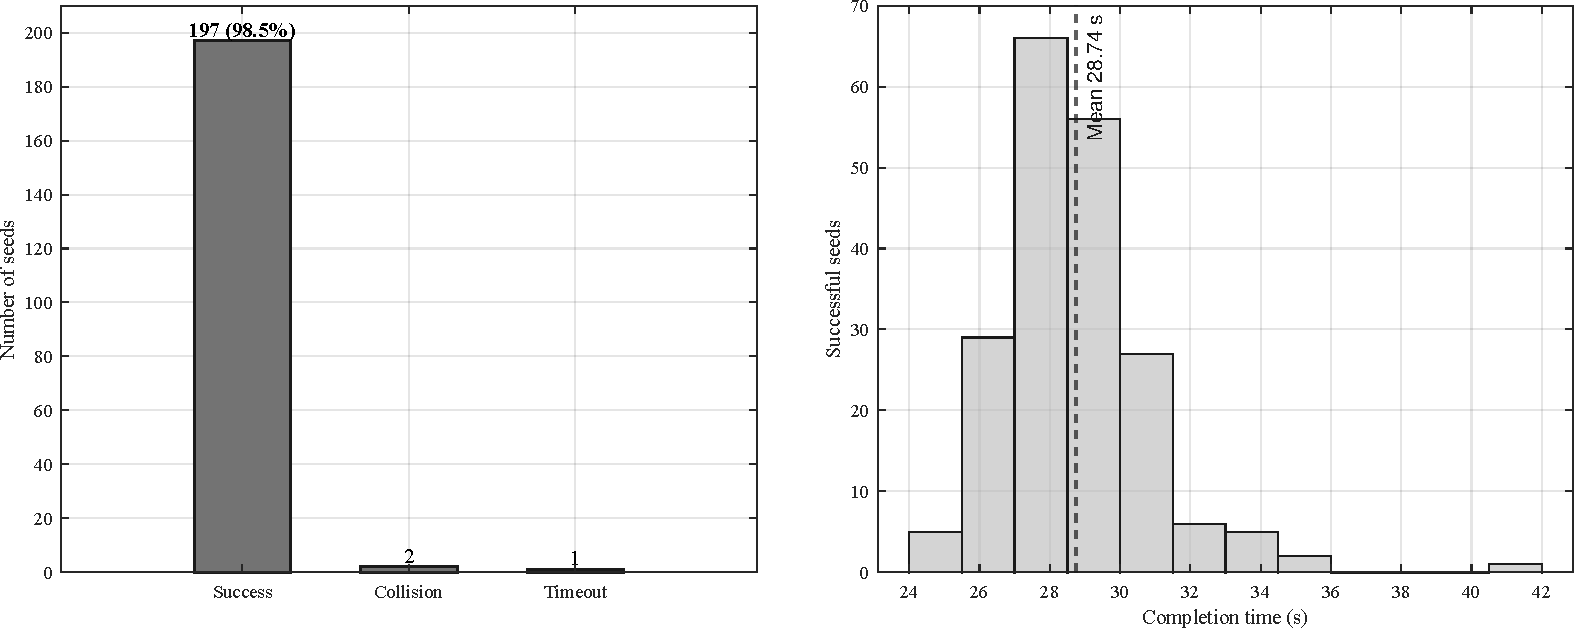
\includegraphics[width=0.96\textwidth]{performance_overview.pdf}
\caption{seed 1--200 的任务结果与成功样本完成时间分布}
\label{fig:performance}
\end{figure}

200 个 seed 中有 197 个成功、2 个碰撞、1 个超时。样本成功率为 98.5\%，Wilson 95\% 区间为 95.68\%--99.49\%。成功任务的平均完成时间为 \SI{28.74}{s}，中位数为 \SI{28.40}{s}，P95 为 \SI{32.36}{s}，最长为 \SI{41.75}{s}。

\begin{table}[H]
\centering
\caption{失败 seed 及结束原因}
\label{tab:failures}
\begin{tabularx}{0.9\textwidth}{@{}C{2.0cm}C{2.8cm}C{2.7cm}Y@{}}
\toprule
seed & 类型 & 结束时间 & 说明 \\
\midrule
133 & collision & \SI{9.20}{s} & 高速绕障过程中触发连续碰撞判定 \\
146 & timeout & \SI{500.00}{s} & 时限内未同时满足目标、队形、速度与保持条件 \\
169 & collision & \SI{8.30}{s} & 高速绕障过程中触发连续碰撞判定 \\
\bottomrule
\end{tabularx}
\end{table}

\subsection{避障路径代价与安全裕度}

\begin{figure}[H]
\centering
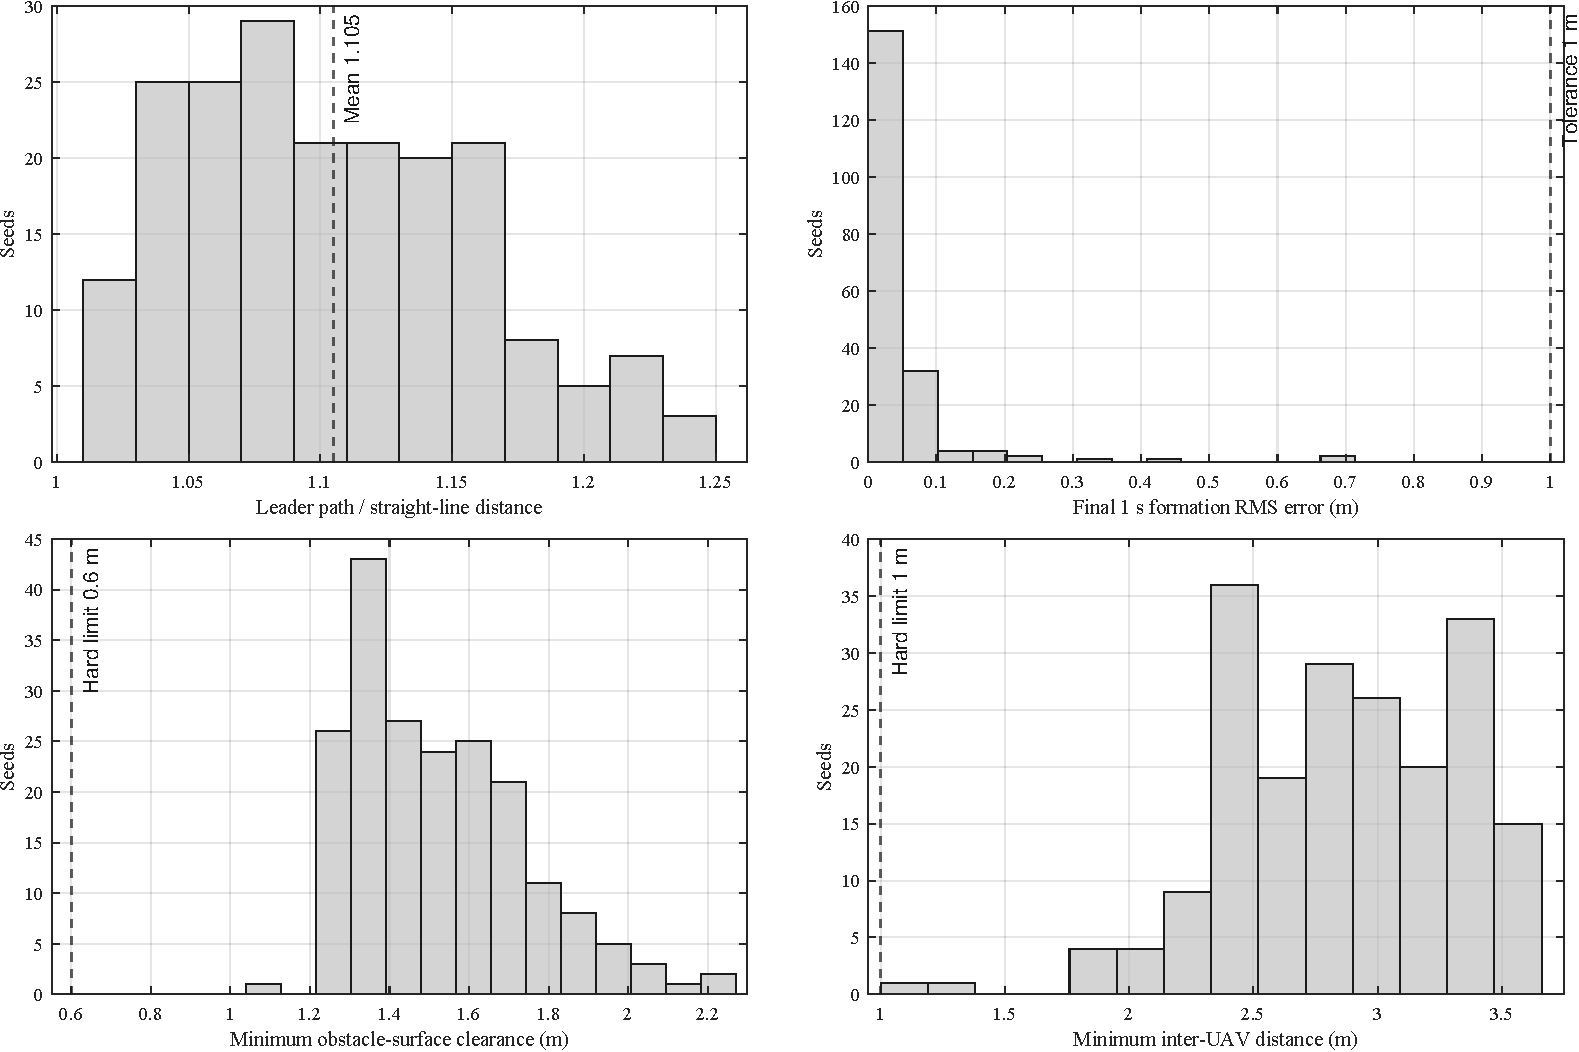
\includegraphics[width=0.98\textwidth]{distribution_metrics.pdf}
\caption{成功 seed 的路径代价、终端队形精度与安全净空分布}
\label{fig:distributions}
\end{figure}

成功 seed 的长机平均路径为 \SI{87.72}{m}，中位数为 \SI{87.36}{m}，P95 为 \SI{95.30}{m}。平均路径代价系数为 1.105，即相对直线距离增加约 10.5\%；P95 代价系数为 1.200。五机平均单机路径为 \SI{93.23}{m}，故一个成功任务的五机累计平均路径约为 \SI{466.13}{m}。

成功 seed 的最小障碍表面距离均值为 \SI{1.525}{m}，最差为 \SI{1.086}{m}，高于 \SI{0.6}{m} 硬阈值；最小机间距离均值为 \SI{2.860}{m}，最差为 \SI{1.099}{m}，只比 \SI{1.0}{m} 硬阈值高 \SI{0.099}{m}。少数场景的机间安全裕度已经很窄，继续提高速度上限需要配套制动距离或速度调度。

\subsection{队形保持误差}

\begin{figure}[H]
\centering
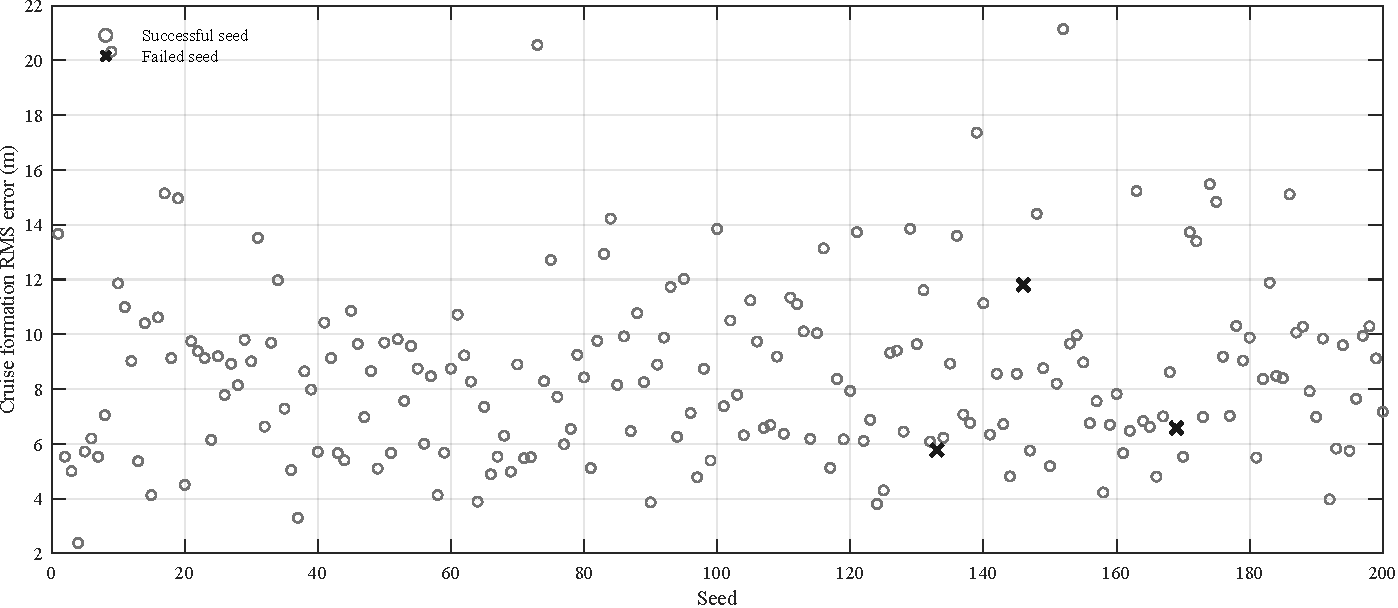
\includegraphics[width=0.96\textwidth]{seed_scatter.pdf}
\caption{各 seed 的巡航队形 RMS 误差}
\label{fig:formation}
\end{figure}

队形误差采用“每一时刻四架僚机最大跟踪误差”的严格口径。成功 seed 的全程逐 seed RMS 均值为 \SI{7.76}{m}，巡航阶段为 \SI{8.59}{m}；全程逐 seed 时间 P95 的均值为 \SI{12.94}{m}。相对 \SI{3}{m} 纵向间距和 \SI{2.5}{m} 横向偏移，该误差不能视为小扰动，表明飞行过程中 V 形几何没有被紧密保持。

另一方面，成功 seed 最后 \SI{1}{s} 的逐 seed RMS 均值只有 \SI{0.062}{m}，最终时刻最大队形误差均值为 \SI{0.054}{m}，跨 seed 的 P95 为 \SI{0.167}{m}。因此，当前设计更准确的描述是“安全走廊跟随并在终点重构 V 形”，而非“全航程刚性 V 形保持”。

\subsection{代表性轨迹与闭环响应}

\begin{figure}[H]
\centering
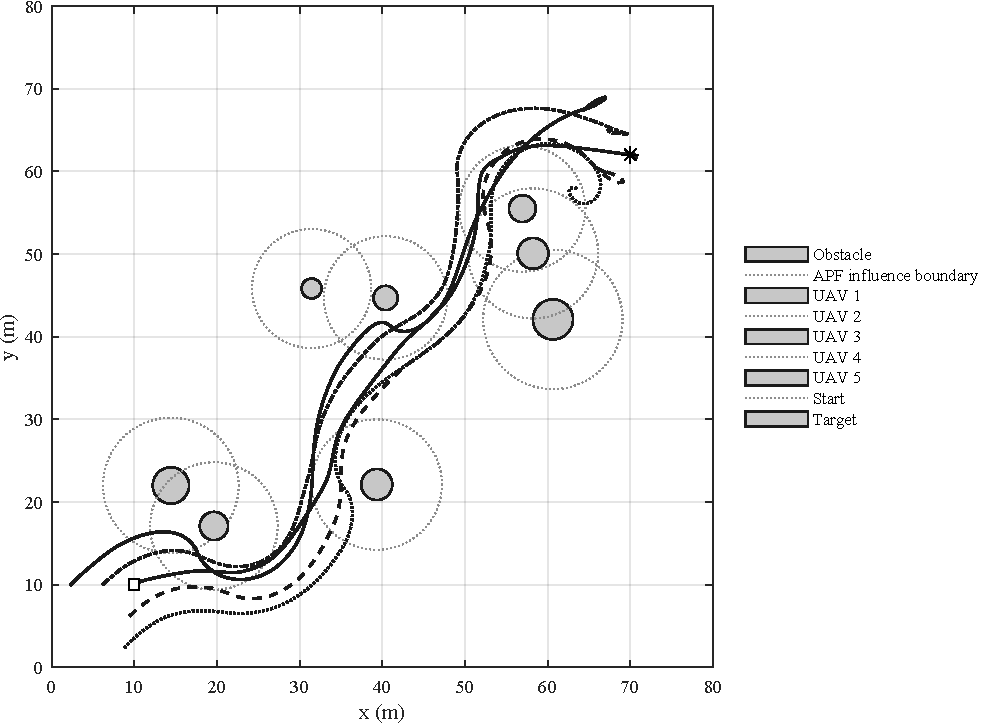
\includegraphics[width=0.82\textwidth]{seed61_trajectory.pdf}
\caption{seed 61 的五机轨迹；灰色实心圆为障碍物，虚线圆为 APF 作用边界}
\label{fig:trajectory}
\end{figure}

seed 61 在 \SI{31.25}{s} 完成任务，长机路径 \SI{93.37}{m}，路径代价系数 1.176，最小障碍表面距离 \SI{1.507}{m}，最小机间距离 \SI{2.347}{m}。其巡航队形 RMS 误差为 \SI{10.71}{m}，最后 \SI{1}{s} RMS 误差为 \SI{0.042}{m}。轨迹显示僚机大体沿同一走廊通过障碍，随后在目标附近恢复固定 V 形。

\begin{figure}[H]
\centering
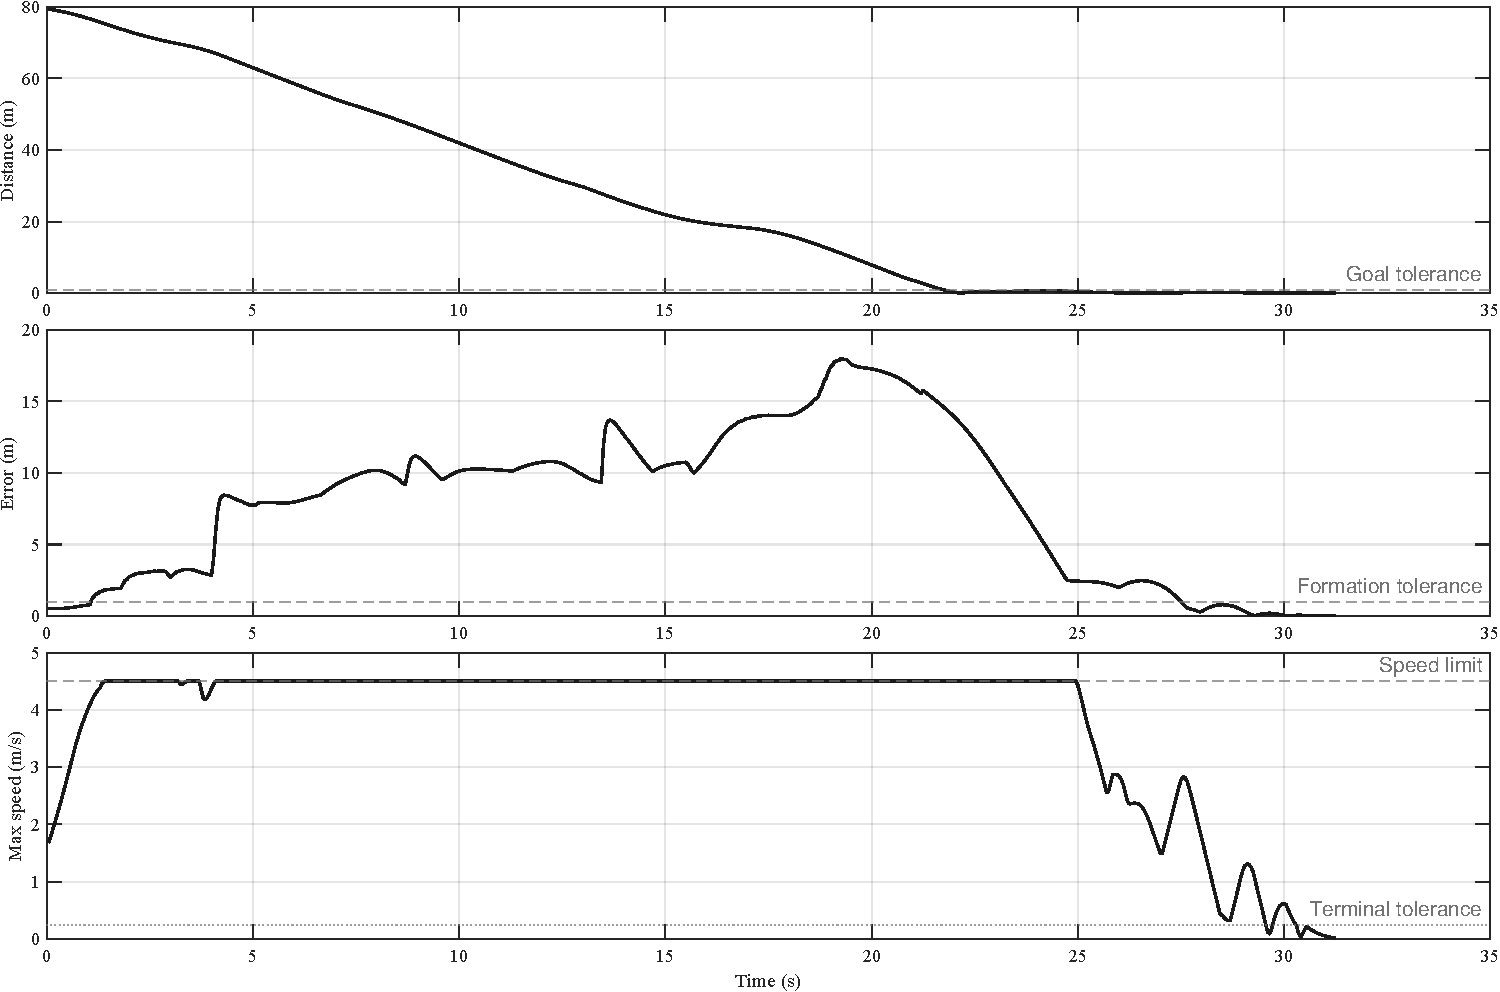
\includegraphics[width=0.97\textwidth]{seed61_response.pdf}
\caption{seed 61 的目标距离、队形误差与最大速度响应}
\label{fig:response}
\end{figure}

seed 61 的最大速度长时间贴近 \SI{4.5}{m/s} 限制，表明速度上限是巡航阶段的活跃约束。队形误差随绕障和参考轨迹切换升高；长机到达目标附近后再用约 \SI{10.05}{s} 完成僚机归队、全机减速和 \SI{1}{s} 连续保持。

\section{闭环稳定性与超调量}

\subsection{局部线性分析}

在无障碍、无机间作用、无输入饱和、ADP 修正冻结且参考位置固定的条件下，僚机位置误差满足
\begin{equation}
\ddot{\bm e}+k_{\mathrm d}\dot{\bm e}+k_{\mathrm p}\bm e=\bm 0.
\end{equation}
取 $k_{\mathrm p}=2.6$、$k_{\mathrm d}=1.8$，得到自然频率 $\omega_n=1.612\,\mathrm{rad/s}$、阻尼比 $\zeta=0.558$ 和极点 $-0.9\pm\mathrm{j}1.338$，极点实部为负。对应标准二阶单位阶跃的理论超调量为 12.08\%，2\% 调节时间约为 \SI{4.44}{s}。

长机保持模式满足
\begin{equation}
\ddot{\bm e}_L+4\dot{\bm e}_L+6\bm e_L=\bm 0,
\end{equation}
其自然频率为 $2.449\,\mathrm{rad/s}$，阻尼比为 0.816，极点为 $-2\pm\mathrm{j}1.414$。标准二阶理论超调量为 1.18\%，2\% 调节时间约为 \SI{2.00}{s}。

\begin{table}[H]
\centering
\caption{局部线性子系统的动态参数}
\label{tab:stability}
\begin{tabularx}{0.94\textwidth}{@{}lC{2.0cm}C{2.6cm}C{3.0cm}Y@{}}
\toprule
子系统 & 阻尼比 & 理论阶跃超调 & 理论 2\% 调节时间 & 适用边界 \\
\midrule
僚机编队 PD & 0.558 & 12.08\% & \SI{4.44}{s} & 固定参考、无障碍、未饱和局部模型 \\
长机目标保持 & 0.816 & 1.18\% & \SI{2.00}{s} & 保持模式下的未饱和局部模型 \\
\bottomrule
\end{tabularx}
\end{table}

\subsection{完整闭环的实证结论}

完整系统是带状态限幅、规划器、停滞逃逸、模式切换、非光滑碰撞修正和在线 ADP 更新的混合非线性闭环，局部 PD 极点不能直接推出全局稳定。在本次 197 个成功 seed 中，所有状态保持有限并最终连续满足目标、队形和速度条件，构成经验收敛证据；3 个失败 seed 则说明闭环尚不具备全场景收敛与安全保证。

经验目标轴向超调均值为 \SI{0.578}{m}，占起终点直线距离的 0.728\%；P95 为 \SI{0.934}{m}，最大为 \SI{1.248}{m}。长机首次进入 \SI{3}{m} 保持触发区至任务成功的平均时间为 \SI{9.39}{s}，P95 为 \SI{12.43}{s}。该时间包括僚机归队、全机减速及 \SI{1}{s} 连续保持，不能与单一二阶环节的理论调节时间等同。

因此，当前项目可以报告“局部线性子系统渐近稳定，Monte Carlo 样本中 98.5\% 收敛”，但不应写成“完整 APF--ADP 编队系统已证明全局渐近稳定”。

\section{环境复杂度与算法复杂度}

\subsection{环境复杂度}

\begin{table}[H]
\centering
\caption{环境复杂度与规划负载}
\label{tab:environment}
\begin{tabularx}{0.95\textwidth}{@{}lC{4.2cm}Y@{}}
\toprule
维度 & 默认值或实测值 & 解释 \\
\midrule
空间规模 & \SI{80}{m}$\times$\SI{80}{m} & 二维有界工作空间，共 \SI{6400}{m^2} \\
障碍规模 & 8 个圆，半径 \SIrange{1.2}{2.6}{m} & 沿起终点走廊随机分布 \\
横向散布 & 直线路径两侧 $\pm\SI{14}{m}$ & 形成具有绕行选择的场景 \\
物理面积占比 & 成功 seed 均值 1.45\% & 障碍实体圆面积之和 \\
\SI{4.2}{m} 膨胀负载 & 均值 14.58\% & 长机路径规划的名义占用指数 \\
\SI{5.6}{m} 有效筛选负载 & 均值 22.04\% & 整队通道可行性筛选指数 \\
直线通道被挡 & 199/200 seed & 按 \SI{4.2}{m} 净空检查 \\
时间上限 & 10000 个离散步 & \SI{500}{s} 除以 \SI{0.05}{s} \\
\bottomrule
\end{tabularx}
\end{table}

面积占比中的膨胀圆未扣除相互重叠，也未扣除越出工作空间边界的部分，因此它是规划负载指标，而不是可通行面积的精确比例。199/200 个场景的直线通道在 \SI{4.2}{m} 净空下被阻挡，说明绝大多数场景确实要求长机绕行。

\subsection{算法复杂度}

记无人机数为 $N$，障碍物数为 $M$，栅格节点数为 $G$，安全层迭代上限为 $I$，仿真步数为 $T$。默认值为 $N=5$、$M=8$、$G=81\times81=6561$、$I\leq5$、$T\leq10000$。

\begin{table}[H]
\centering
\caption{主要模块的渐近复杂度}
\label{tab:complexity}
\small
\begin{tabularx}{\textwidth}{@{}lC{4.5cm}Y@{}}
\toprule
模块 & 时间或空间复杂度 & 默认规模下的主要负担 \\
\midrule
占据栅格生成 & $O(GM)$ & 每个障碍更新 6561 个栅格点 \\
栅格建图与最短路 & $O(G+E)$ 建图，$O((G+E)\log G)$ 搜索 & 八邻接稀疏图，$E$ 与 $G$ 同阶 \\
每步 APF 与机间斥力 & $O(NM+N^2)$ & 5 架机遍历 8 个障碍和 10 对机间关系 \\
每步预测安全层 & $O(I(NM+N^2))$ & 最多 5 轮障碍及机间扫掠修正 \\
每步 ADP & $O(Nd)$ & 特征维数 $d=6$，另含二维有限差分 \\
历史记录 & $O(TN)$ 空间 & 保存状态和指标，最多 10000 步 \\
\bottomrule
\end{tabularx}
\end{table}

终端归队阶段，每架僚机还可能单独调用栅格规划；当目标变化或路径为空时，最快每 \SI{2}{s} 重规划一次。系统扩展到更多无人机时，$N^2$ 机间项、安全层多轮预测和多僚机局部规划将成为主要计算瓶颈。

\section{约束条件与适用范围}

\begin{itemize}
  \item 当前模型为二维质点，不包含姿态、推力方向、执行器动态、电池、气动力、风场和三维高度分层。
  \item 障碍物静止且为圆形；没有动态障碍、感知噪声、定位漂移、通信延迟、丢包或异步更新。
  \item 控制器默认已知全部障碍物中心和半径，长机轨迹可由全部僚机无延迟访问。
  \item 场景先经过 \SI{5.6}{m} 有效净空筛选，因此结果没有覆盖窄通道不可通行、无可行整队路径或场景生成失败的概率。
  \item 碰撞安全层是在有限步长和有限加速度下的启发式预测修正，不能替代形式化安全证明。
  \item ADP 权重有范数上限，可以避免数值爆炸，但没有持续激励、策略最优性或权重收敛保证。
  \item 成功率只反映当前参数和 seed 1--200；Wilson 区间表示该样本下的统计不确定性，不能推广为真实飞行安全概率。
  \item \SI{4.5}{m/s} 上限在所有成功 seed 中都被触及，说明速度约束主导巡航阶段；进一步提速会增大制动距离和稀有碰撞风险。
\end{itemize}

\section{结论与后续建议}

当前 V1.1.1 已形成完整的随机场景生成、路径规划、APF 避障、ADP 在线修正、领航--跟随编队、预测式安全层、失败诊断和批量复现流程。在 200 个固定 seed 中，系统以 \SI{28.74}{s} 的成功样本平均时间和 10.5\% 的平均长机路径增量完成了 98.5\% 的任务，终点归队精度较高。

项目当前最明显的问题不是终点精度，而是巡航阶段的队形保持。\SI{8.59}{m} 的巡航 RMS 误差与 V 形尺度相当甚至更大；轨迹跟随策略还使多机倾向从障碍物同一侧通过。因此，如果研究目标强调“全过程队形保持与柔性变形”，需要在参考队形层增加可控形变或分流--汇合机制，而不能只继续增大 PD 增益。

建议按以下顺序继续工作：
\begin{enumerate}
  \item 复盘 seed 133 和 169 的碰撞时刻，按剩余净空和路径曲率调节最大速度，使 \SI{4.5}{m/s} 成为条件上限，而不是全程硬顶。
  \item 把编队参考从单一长机轨迹扩展为弹性编队或多走廊分配，允许部分僚机从障碍物另一侧绕行，并在通过后用有界时间重新汇合。
  \item 为巡航队形误差设独立指标和上限，同时报告全程 RMS、巡航 RMS、末段 RMS 与最大误差，避免最终误差掩盖中途形变。
  \item 补充 APF、ADP、安全层和规划净空的消融实验，区分各模块对成功率、路径代价、控制代价和队形误差的贡献。
  \item 若需要论文级稳定性结论，应建立包含模式切换和输入饱和的误差系统，给出 Lyapunov 或 ISS 条件，并对 ADP 近似误差和安全层扰动给出界。
  \item 进入实机前增加三维动力学、风扰、感知误差、通信延迟、动态障碍和执行器带宽，再进行硬件在环与低速室内试验。
\end{enumerate}

\appendix

\section{关键参数}

\begin{longtable}{@{}lC{3.0cm}p{8.0cm}@{}}
\caption{V1.1.1 关键参数}\label{tab:parameters}\\
\toprule
参数 & 数值 & 作用 \\
\midrule
\endfirsthead
\toprule
参数 & 数值 & 作用 \\
\midrule
\endhead
$\Delta t$ & \SI{0.05}{s} & 积分与控制周期 \\
$T_{\max}$ & \SI{500}{s} & 单任务时间上限 \\
$v_{\max}$ & \SI{4.5}{m/s} & 速度幅值上限 \\
$a_{\max}$ & \SI{3.0}{m/s^2} & 加速度幅值上限 \\
\code{pathClearance} & \SI{4.2}{m} & 长机规划障碍膨胀净空 \\
场景有效净空 & \SI{5.6}{m} & 整队通道可行性筛选的实际净空 \\
$\rho_0$ & \SI{6.0}{m} & 障碍斥力作用范围 \\
\code{obsSafe} & \SI{0.6}{m} & 障碍硬碰撞安全距离 \\
\code{uavSafe} & \SI{1.0}{m} & 机间硬碰撞距离 \\
\code{uavAvoidSafe} & \SI{3.0}{m} & 机间斥力启动距离 \\
\code{goalTol} & \SI{1.0}{m} & 长机终点容差 \\
\code{formTol} & \SI{1.0}{m} & 终端最大队形误差容差 \\
\code{vTol} & \SI{0.25}{m/s} & 终端最大速度容差 \\
\code{holdDuration} & \SI{1.0}{s} & 成功条件连续保持时间 \\
ADP gain / $u_{\max}$ & 0.5 / 0.8 & 在线修正缩放与 Actor 输出限制 \\
ADP $\gamma$ & 0.95 & 长期代价折扣 \\
\bottomrule
\end{longtable}

\begingroup
\small
\setstretch{1.15}
\section{复现信息}

\begin{itemize}
  \item 源码目录：F 盘 \nolinkurl{UAV_APF_ADP_Formation} 项目根目录。
  \item 源码版本：V1.1.1，Git 提交 \code{5f5b69c2214c40c0e8ccf05cc6e1401fd63f860a}。
  \item 核心入口：\nolinkurl{config/default_params.m}、\nolinkurl{src/run_simulation.m}、\\
  \nolinkurl{src/leader_control.m}、\nolinkurl{src/follower_control.m}、\nolinkurl{src/plan_grid_path.m}。
  \item 评估数据：附件 Seed 1--200 指标表（CSV），每行对应一个 seed，包含结果、时间、路径、误差、净空、速度、控制量与环境负载指标。
  \item 验证结果：项目自带 11 项核心测试全部通过；seed 1--200 已逐一运行，无缺失记录。
  \item 统计日期：2026 年 9 月 22 日，时区 Asia/Shanghai。
\end{itemize}

\section{统计口径补充说明}

报告中的均值、分位数与极值以 seed 为统计单位。队形 RMS 先在每个 seed 的时间序列上计算，再对 seed 汇总，因此每个场景权重相同，不会让运行时间更长的场景自动占据更高权重。

膨胀面积比例是各障碍膨胀圆面积之和除以工作空间面积，未扣除重叠，也没有扣除越出边界的部分，适合比较规划负载，不应作为可通行面积的精确比例。

目标轴向超调与经典二阶阶跃超调的定义不同。前者是任务轨迹几何量，后者来自理想化局部线性模型；两者用于分别说明实际终点越界和局部动态特性，不作一一对应。

\endgroup
\end{document}
